\documentclass{beamer}
%
% Choose how your presentation looks.
%
% For more themes, color themes and font themes, see:
% http://deic.uab.es/~iblanes/beamer_gallery/index_by_theme.html
%
\mode<presentation>
{
  \usetheme{default}      % or try Darmstadt, Madrid, Warsaw, ...
  \usecolortheme{default} % or try albatross, beaver, crane, ...
  \usefonttheme{default}  % or try serif, structurebold, ...
  \setbeamertemplate{navigation symbols}{}
  \setbeamertemplate{caption}[numbered]
  %\setbeamertemplate{footline}[frame number]
}
\usepackage{outlines}
 
\usepackage{graphicx}
\usepackage[english]{babel}
\usepackage[utf8x]{inputenc}
\title{Modeling Module 1}
\setbeamertemplate{footline}[frame number]
%\author{Instructor; M.K. Srivas \\
%TA: Zubin Duggal}

\begin{document}
\begin{frame}
  \titlepage
\end{frame}

% Uncomment these lines for an automatically generated outline.
%\begin{frame}{Outline}
%  \tableofcontents
%\end{frame}

\section{Outline}


\begin{frame}{Outline}
\begin{itemize}
\item What's a Model?

\item State-Transition Systems (TS)

\item Abstraction and Non-determinism in Modeling

\item Modeling Examples

\item Kripke Structures, Behaviors of TS
\end{itemize}
\end{frame}

\begin{frame}{Model Checking: Cited for Turing Award in 2007 \\
(Invented: 1986)}
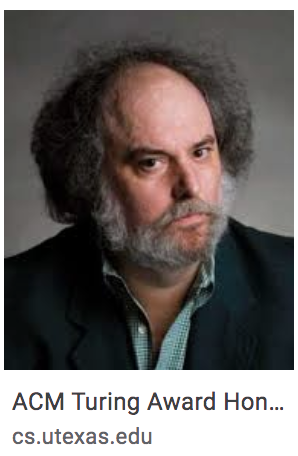
\includegraphics[scale=0.4]{pics/allen.png}\hfill
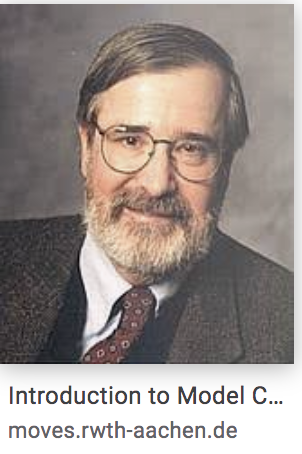
\includegraphics[scale=0.4]{pics/clarke.png}\hfill
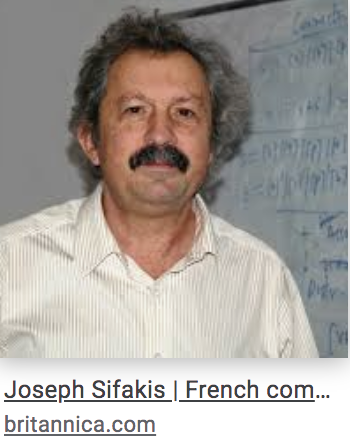
\includegraphics[scale=0.4]{pics/sifakis.png}

E. Allen Emerson~~~~~~~~~~~Edmund Clarke~~~~~~~~~~~~Joseph Sifakis
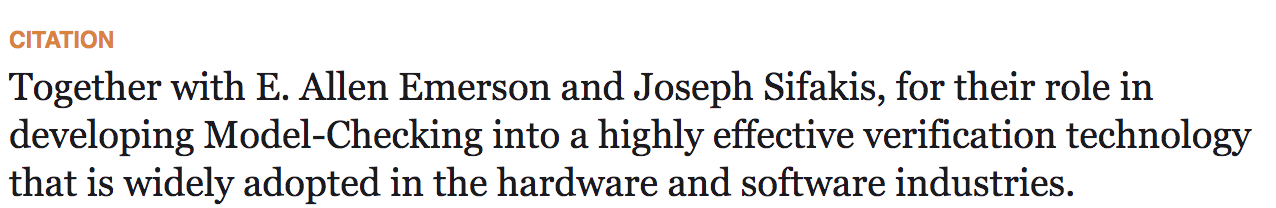
\includegraphics[scale=0.5]{pics/Citation.png} 
\end{frame}

\begin{frame}{What Kind of Systems and Properties?}
\uncover<1->{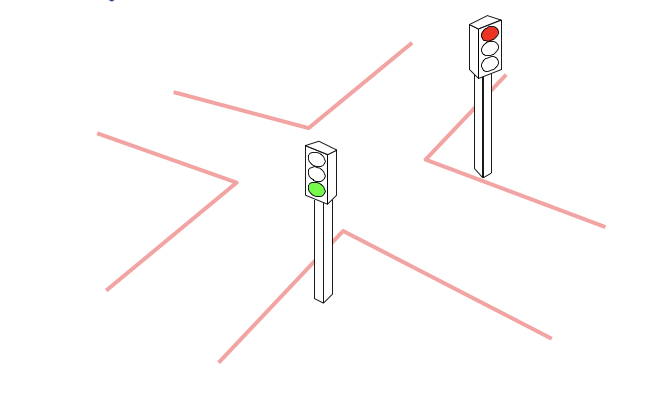
\includegraphics[scale=0.3]{pics/trafficsignal.png}}\hfill
\uncover<3->{\includegraphics[scale=0.2]{pics/mod3cnt.png}}\\
\uncover<2->{\tiny{``traffic lights should never be green at the same time''}} \hfill
\uncover<4->{\tiny{``the counter value (`ab') is always $\leq$ 3''}}
\vfill
\uncover<5->{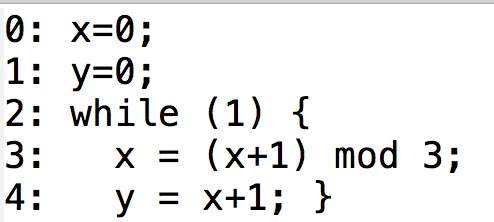
\includegraphics[scale=0.3]{pics/code.png}}\hfill
\uncover<7->{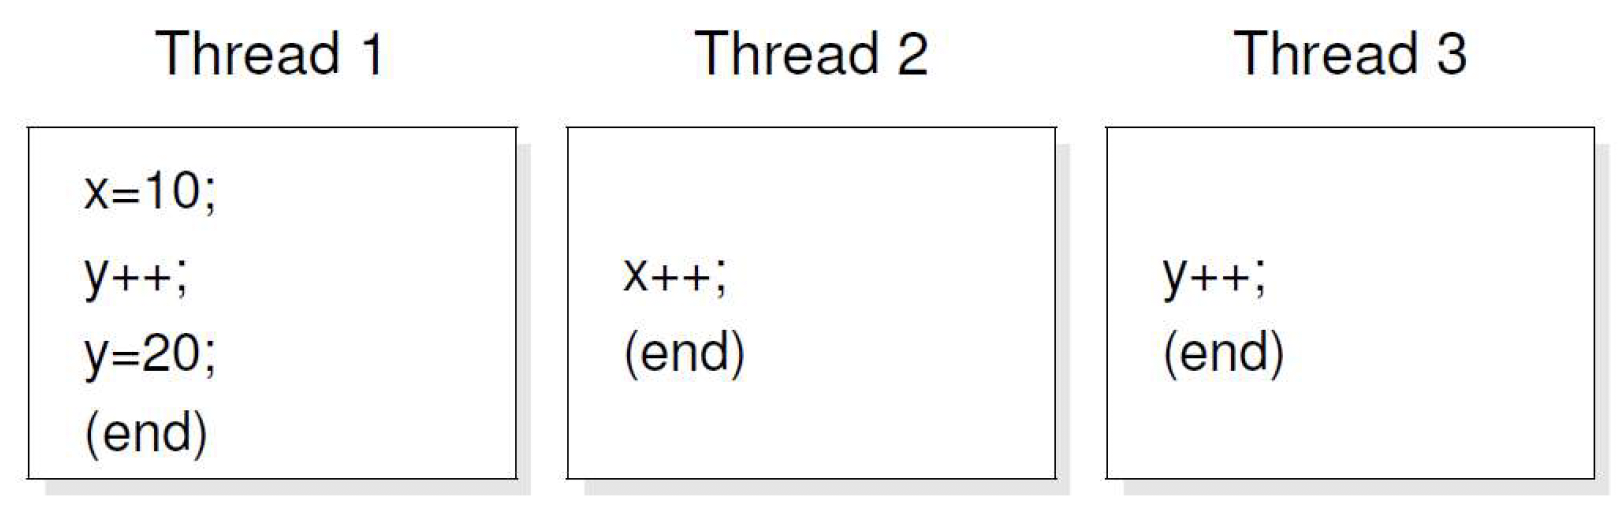
\includegraphics[scale=0.15]{pics/concprog.png}}\\
\uncover<6->{\tiny{``@line~3: $y \geq x$ $always$ holds''}} \hfill
\uncover<8->{\tiny{``the program has no data races''}} \\
\uncover<6->{\tiny{``@line~3: x=0 holds infinitely often''}}

\end{frame}

\begin{frame}{What Kind of Systems Not} 
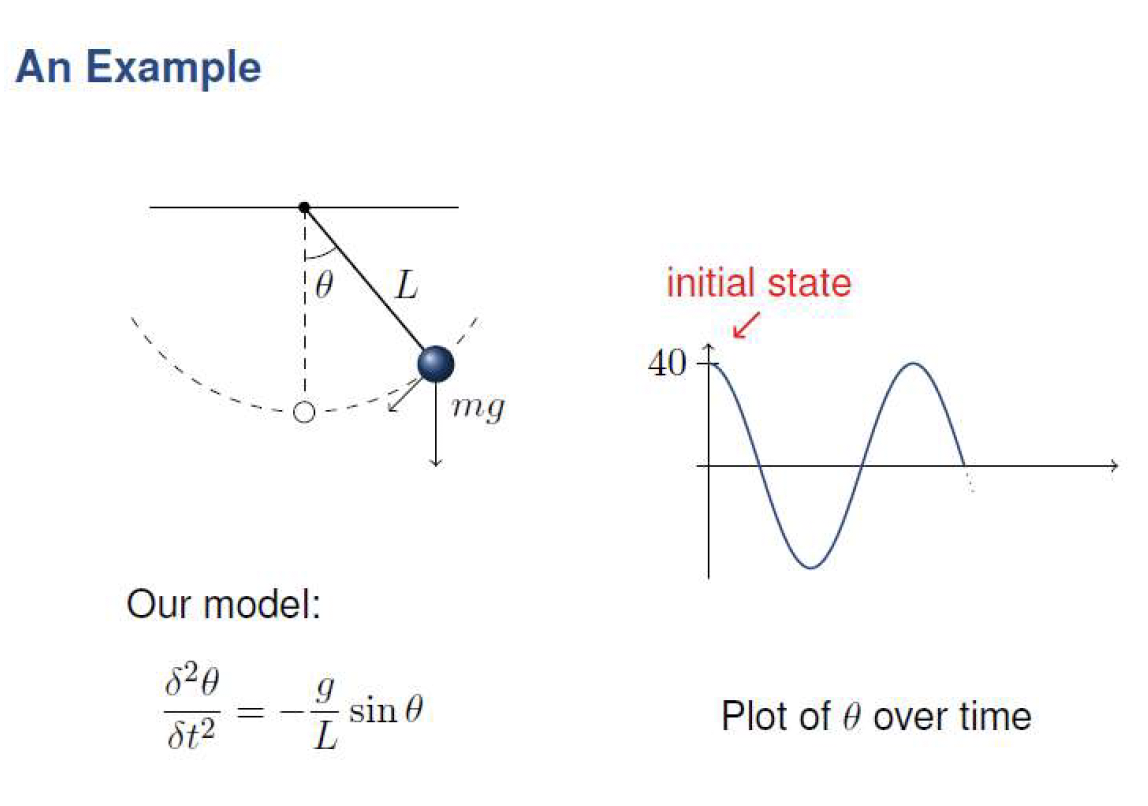
\includegraphics[scale=0.3]{pics/contdynamics.png}
\end{frame}

\begin{frame}{What do we need for formal verification?}
\begin{itemize}
\item<1-> Need a common formalism to model all systems of interest:
\textbf{Transition Systems (M)}

\item<2-> Need an expressive logic/language to specify desired properties \\
\textbf{``Special-purpose Temporal Logics (Prop)''}

\item<3-> Need efficient algorithms to automatically check properties \\
\textbf{M $\models$ Prop}
\end{itemize}
\end{frame}

\begin{frame}{A Hardware Abstraction Example}
\uncover<1->{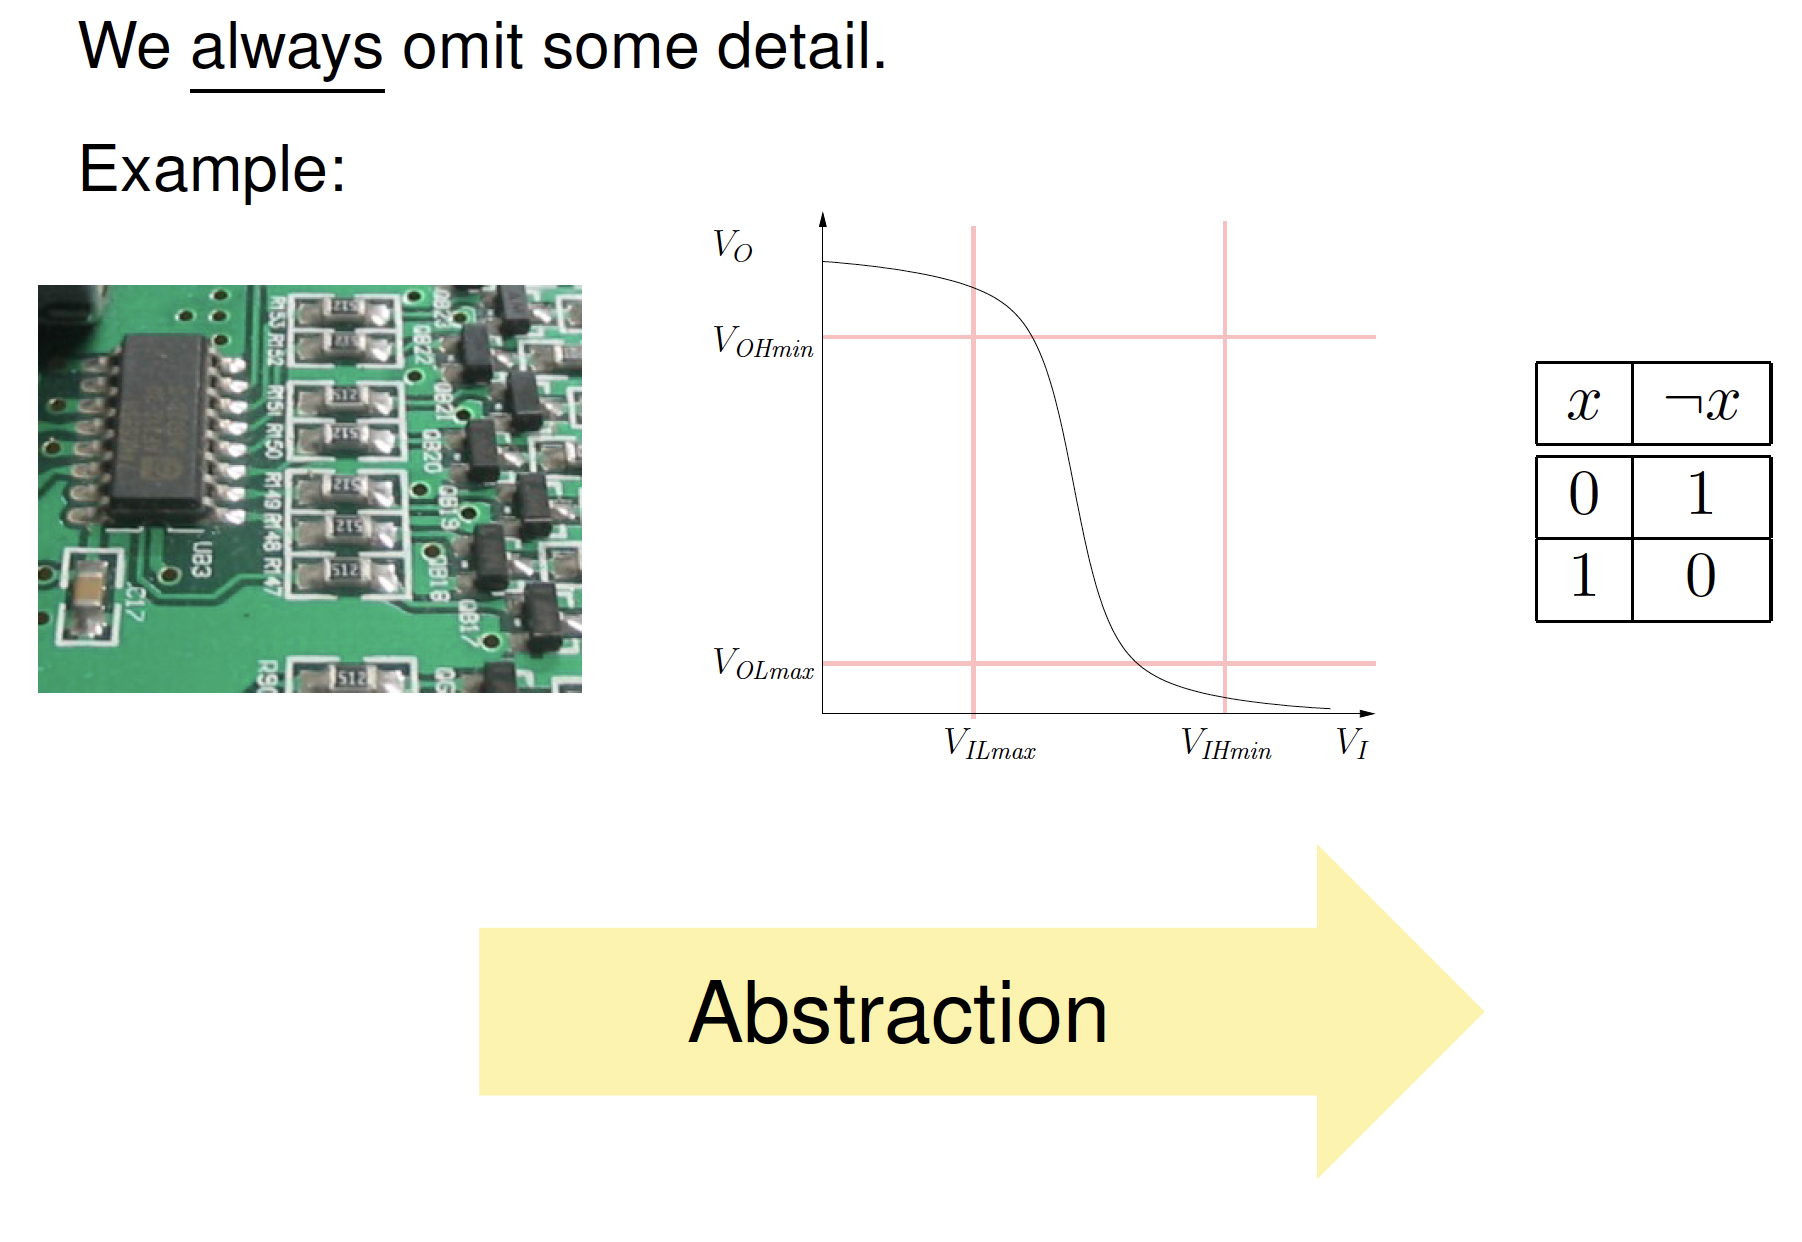
\includegraphics[scale=0.3]{pics/HWabs.png}}
\end{frame}

\begin{frame}{Modeling: States}
\begin{itemize}
\item<1-> Our systems have a state, \\
the model has a set of states

\item<2-> This is typically given as a valuation of state variables
\begin{itemize}
\item $\theta$
\item Velocity
\item Data stored in program variables
\item Data stored in hardware registers/flip-flops
\item ....
\end{itemize}

\item<3-> We focus on \underline{discrete state variables}
\end{itemize}
\end{frame}

\begin{frame}{Modeling State Transitions}
\begin{itemize}
\item<1-> When the state changes with time, \\
we have a \underline{state transition}

\item<2-> Time can be modeled as
 \begin{itemize}
\item continuous
\item discrete
\end{itemize}

\item<3-> We will focus on discrete-time transitions
\end{itemize}
\end{frame}

\begin{frame}{Definition Transition System}
Definition (Transition System) \\
A $Transition~System$ is a 3-tuple $M = (S, S_0, T)$ consisting of
\begin{itemize}
\item a set of states $S$,

\item a set of initial states $S_0 \subseteq S$\item a transition relation $T \subseteq (S X S)$
\end{itemize}
\end{frame}

\begin{frame}{Modeling Sequential Code: An Example}
\uncover<1->{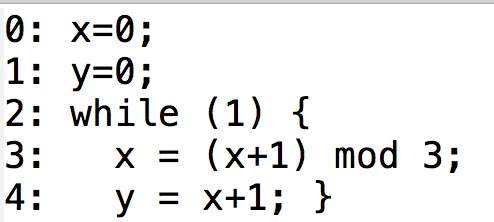
\includegraphics[scale=0.3]{pics/code.png}}\hfill
\uncover<2->{\includegraphics[scale=0.3]{pics/xymodprogcfg.png}} \\
\uncover<3->{\includegraphics[scale=0.25]{pics/xymodprogTS1.png}} \\
\uncover<3->{\tiny{$TS:~M = (S, S_0, R)$}}
\begin{itemize}
\item<3-> $S = (D_1 X D_2)$, where $D_1 = \{0,1,2\}, D_2 = \{0,1,2,3\}$
\item<3-> $S_0 = \{(0,0)\}$
\item<3-> $R = \{ ((0,0),(1,2)), ((0,1),(1,2)), ((1,2),(2,3)), ((2,3),(0,1))  \}$
\end{itemize}
\end{frame}

\begin{frame}{Towards Symbolic Representation for TS:\\
Notation for States}
\begin{itemize}
\item $S$ - set of states

\item $s \in S$ - one particular state

\item $s,x$ - the value of some variable $x$ in state $s$. \\
These are called \underline{state variables}
\end{itemize}
\end{frame}

\begin{frame}{Towards Symbolic Representation for TS:\\The Transition Relation}
\includegraphics[scale=0.3]{pics/symbolic1.png}
\end{frame}

\begin{frame}{Towards Symbolic Representation for TS:\\Characteristic Functions}
\includegraphics[scale=0.3]{pics/symbolic2.png}
\end{frame}

\begin{frame}{Towards Symbolic Representation for TS:\\The Transition Relation Again}
\includegraphics[scale=0.3]{pics/symbolic3.png}
\end{frame}

\begin{frame}{Symbolic TS for the Code Example}
\uncover<1->{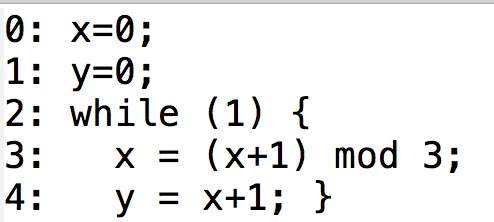
\includegraphics[scale=0.3]{pics/code.png}}\hfill
\uncover<2->{\includegraphics[scale=0.3]{pics/xymodprogcfg.png}} \\
\uncover<3->{\includegraphics[scale=0.25]{pics/xymodprogTS1.png}} \\
\uncover<3->{\tiny{$TS:~M = (S, S_0, R)$}}
\begin{itemize}
\item<3-> $S = (D_1 X D_2)$, where $D_1 = \{0,1,2\}, D_2 = \{0,1,2,3\}$
\item<3-> $S_0(s): (s.x = 0 \land s.y =0)$
\item<3-> $R(s,s'): (s'.x = s.x+1~mod~3) \land (s'.y = s'.x + 1) $
\end{itemize}
\end{frame}

\begin{frame}{Role of Nondeterminism in Modeling}
\begin{itemize}
\item<1-> $Nondeterminism$ is used to abstract, i.e., not deliberately committing, to certain details in modeling systems
\begin{itemize}
\item<2-> Initial nondeterminism: Initial state need not be unique

\item<3-> Inputs (environment) nondeterminism: Inputs can change arbitrarily

\item<4-> Scheduler nondeterminism (concurrent systems): Multiple successor states possible for a transition

\end{itemize}
\end{itemize}
\end{frame}

\begin{frame}{Initial State Nondeterminism}
\uncover<1->{\includegraphics[scale=0.3]{pics/codearb.png}} \\
%\uncover<2->{\includegraphics[scale=0.3]{pics/xymodprogcfg.png}} \\
\uncover<3->{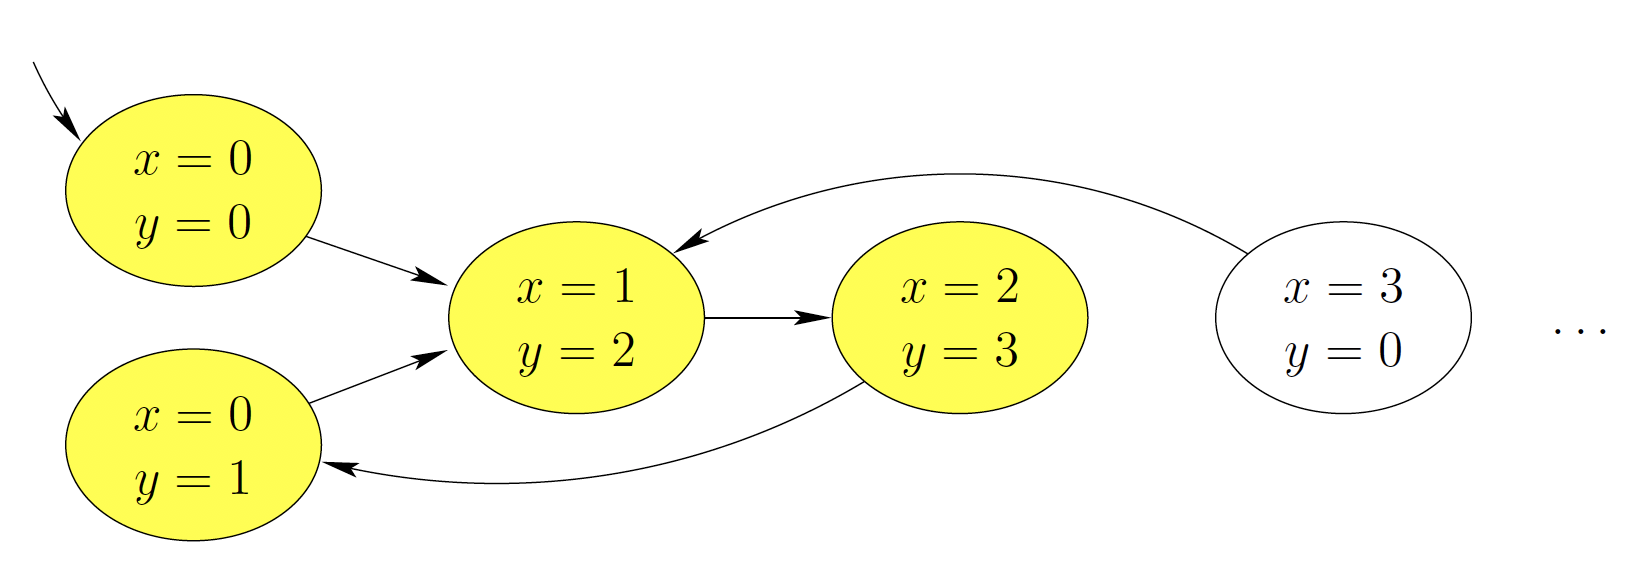
\includegraphics[scale=0.25]{pics/xymodprogTS.png}} \\
\uncover<3->{\tiny{$TS:~M = (S, S_0, R)$}}
\begin{itemize}
\item<3-> $S = (Nat~X~Nat)$
\item<3-> $S_0(s): (s.y = 0)$
\item<3-> $R(s,s'): (s'.x = s.x+1~mod~3) \land (s'.y = s'.x + 1) $
\end{itemize}
\end{frame}

\begin{frame}{Modeling Clocked Hardware: Modulo 4 Counter}
\uncover<1->{\includegraphics[scale=0.3]{pics/mod3cnt.png}}
\begin{itemize}
\item One global clock: $clk$ \\

\item One input: $rst$

\item Next-state logic (dashed box): \\
$a, b$ (flip-flops) change $synchronously$ with every tick of $clk$
\begin{itemize}
\item $\delta(a, b, rst).a \equiv \overline{rst}~.~(a \oplus b)$
\item $\delta(a, b, rst).b \equiv \overline{rst}~.~\overline{b}$
\end{itemize}


\end{itemize}
\end{frame}

\begin{frame}{Modeling Inputs in TS}
\uncover<1->{\includegraphics[scale=0.3]{pics/mod3cnt.png}}\hfill
\uncover<2->{\includegraphics[scale=0.3]{pics/mod3cntTSwithInput.png}} \\
\uncover<3->{\includegraphics[scale=0.3]{pics/inputnondetTS.png}}\hfill $T(s,s') \equiv$ \\
~~~~~~~~~~~~~~~~~~~$(\delta(s.a,s.b, s.rst) = s'.ab \lor$ \\
~~~~~~~~~~~~~~~~~~~$\delta(s.a,s.b,s.rst) = s'.ab$
\end{frame}

\begin{frame}{Assumptions on Transition Systems}
Definition (Transition System) \\
A $Transition~System$ is a 3-tuple $M = (S, S_0, T)$ consisting of
\begin{itemize}
\item a set of states $S$,

\item a set of initial states $S_0 \subseteq S$\item a transition relation $T \subseteq (S X S)$
\end{itemize}

\begin{enumerate}
\item<1-> Domains of state variables are \underline{finite and discrete}

\item<2-> Transition relation is total (No loss of generality)
\begin{itemize}
\item How about terminating systems, e.g., code?
\item If $T(s,s') \equiv false$, then redfeine it as $T'(s,s') \equiv (s=s') $
\end{itemize}
\end{enumerate}
\end{frame}

\begin{frame}{Terminating TS}
\includegraphics[scale=0.3]{pics/terminatingTS.png}
\end{frame}

\begin{frame}{}
\end{frame}

\begin{frame}{}
\begin{itemize}
\item

\end{itemize}
\end{frame}

\begin{frame}{}

\end{frame}

\begin{frame}{An Continuous Domain Example}
\uncover<1->{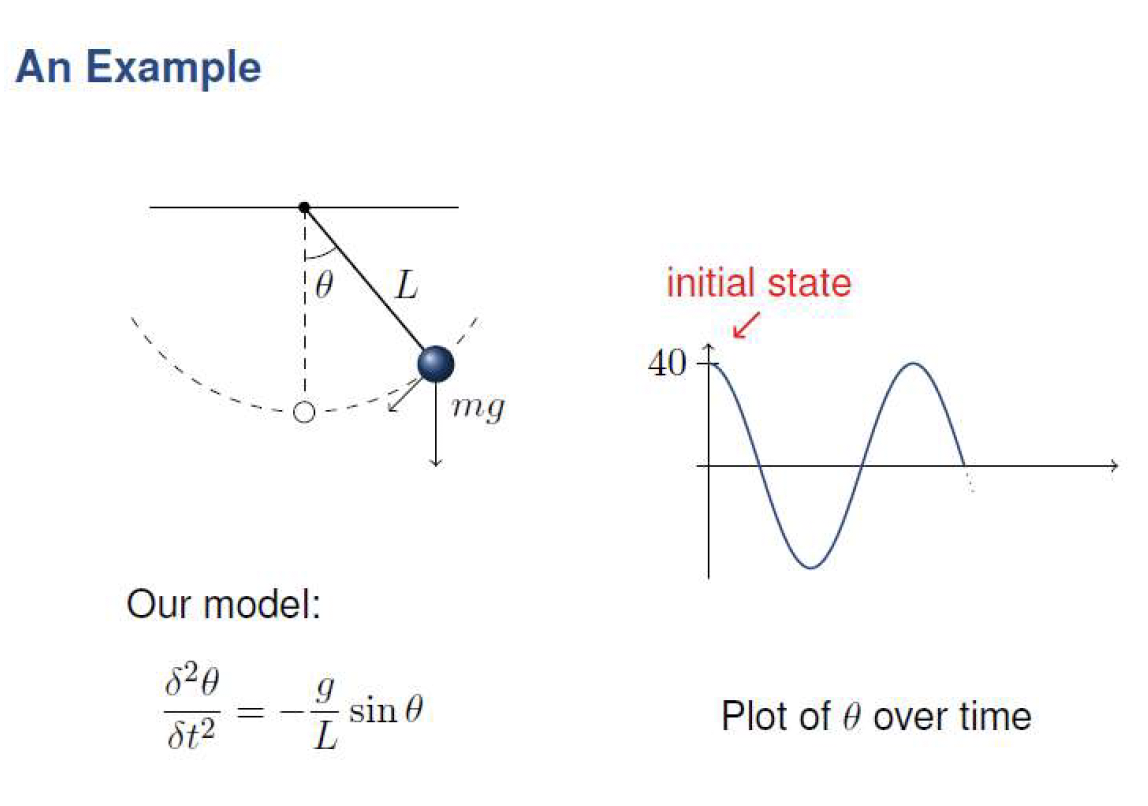
\includegraphics[scale=0.3]{pics/contdynamics.png}}
\end{frame}



\end{document}
